\hsection{Interlude:~Searching in the Python Documentation}%
\label{sec:pythonDocumentation}%
\let\oldinterludepythonglslink\glslink%
\protected\gdef\glslink#1#2{#2}%
%
\begin{figure}%
\centering%
%
\subfloat[][%
We open a browser and visit the \citetitle{PSF:P3D}~\cite{PSF:P3D} at~\citeurl{PSF:P3D}.%
\label{fig:pythondoc01website}%
]{\tightbox{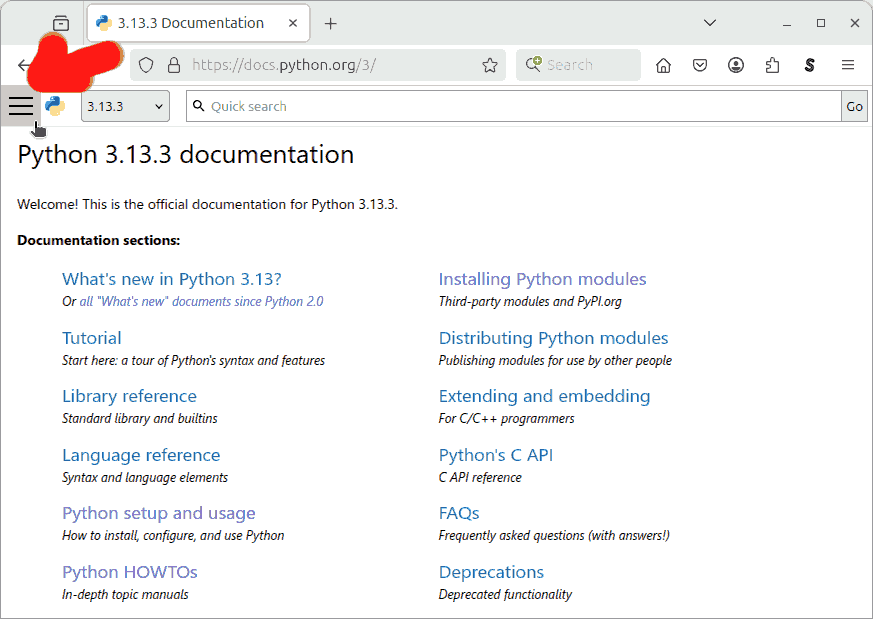
\includegraphics[width=0.47\linewidth]{\currentDir/pythondoc01website}}}%
%
\floatSep%
%
\subfloat[][%
If you click the \menu{\threeBarButton} at on the top-left corner of the website, you can get to a menu where you can change the language and, e.g., select simplified Chinese~(简体中文) if that is your preferred language.~%
(I will not do so and instead continue in English.)%
\label{fig:pythondoc02language}%
]{\tightbox{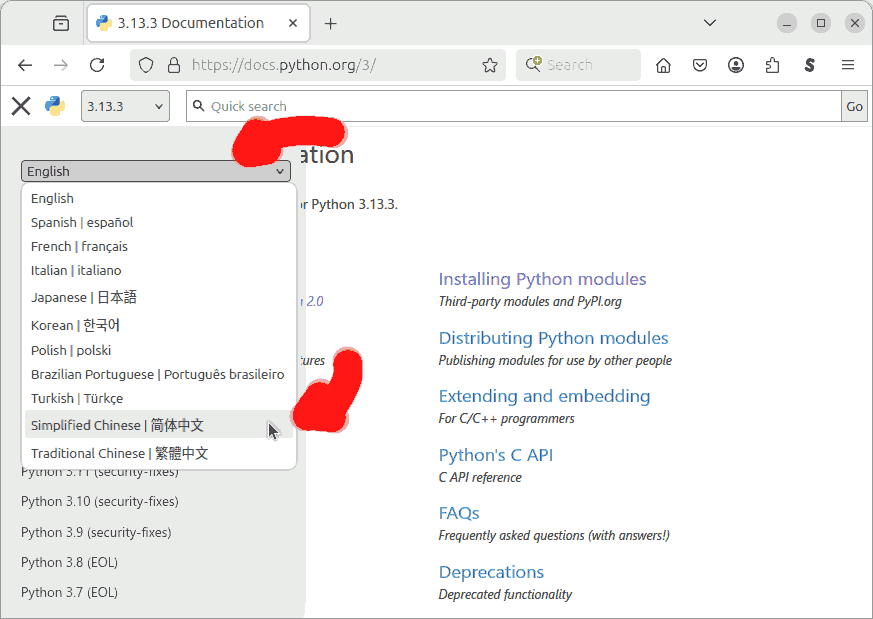
\includegraphics[width=0.47\linewidth]{\currentDir/pythondoc02language}}}%
%
\floatRowSep%
%
\subfloat[][%
We are looking for information on the \pythonilIdx{ceil} function and therefore type \pythonilIdx{ceil} into the search bar \emph{of the website} and click on~\menu{Go}.%
\label{fig:pythondoc03searchCeil}%
]{\tightbox{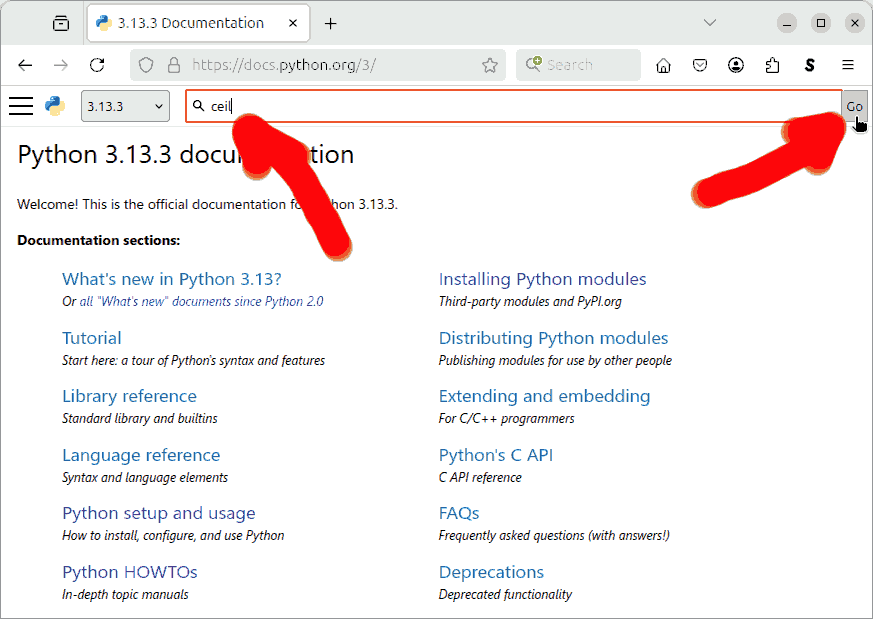
\includegraphics[width=0.47\linewidth]{\currentDir/pythondoc03searchCeil}}}%
%
\floatSep%
%
\subfloat[][%
Especially if you visit the website for the first time in your current web browser session, it may take some time until results show up. %
We wait patiently.%
\label{fig:pythondoc04wait}%
]{\tightbox{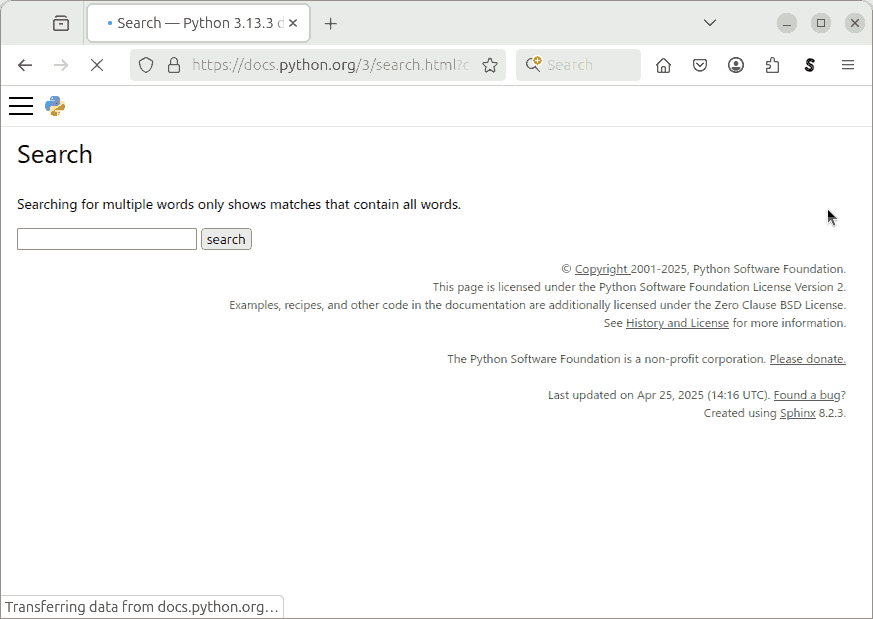
\includegraphics[width=0.47\linewidth]{\currentDir/pythondoc04wait}}}%
%
\floatRowSep%
%
\subfloat[][%
A list of documentation articles about the \pythonilIdx{ceil} function appears. %
We click on the link to~\pythonil{math.ceil}.%
\label{fig:pythondoc05results}%
]{\tightbox{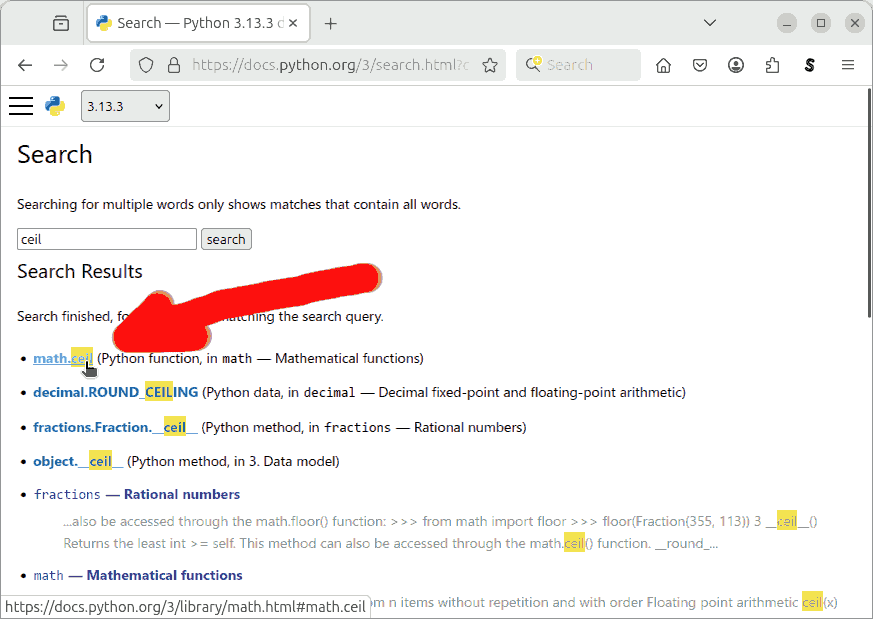
\includegraphics[width=0.47\linewidth]{\currentDir/pythondoc05results}}}%
%
\floatSep%
%
\subfloat[][%
It takes us to the \pythonilIdx{ceil}~entry of the \citetitle{PSF:P3D:TPSL:MMF} page~\cite{PSF:P3D:TPSL:MMF} at \citeurl{PSF:P3D:TPSL:MMF}. %
Indeed, we find a brief explanation about the \pythonilIdx{ceil} function.~%
(Also, we find a link to further reading about the \dunder{ceil} method, which we will discuss much later in~\cref{fig:pythonDunder:2}.)
\label{fig:pythondoc06mathceil}%
]{\tightbox{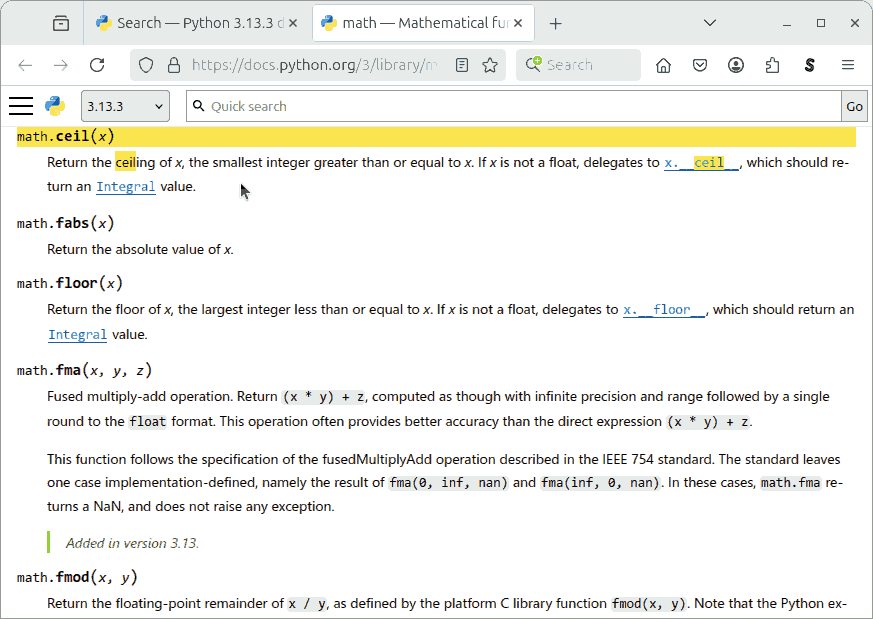
\includegraphics[width=0.47\linewidth]{\currentDir/pythondoc06mathceil}}}%
%
%
\caption{Searching the \citetitle{PSF:P3D}~\cite{PSF:P3D} for information about the function~\pythonilIdx{ceil}.}%
\label{fig:pythondoc:A}%
\end{figure}%
%
\begin{figure}%
\centering%
%
\subfloat[][%
We try searching for information about \inQuotes{round towards positive infinity} in the~\citetitle{PSF:P3D}~\cite{PSF:P3D} at~\citeurl{PSF:P3D}.%
\label{fig:rounding01searchInDocumentation}%
]{\tightbox{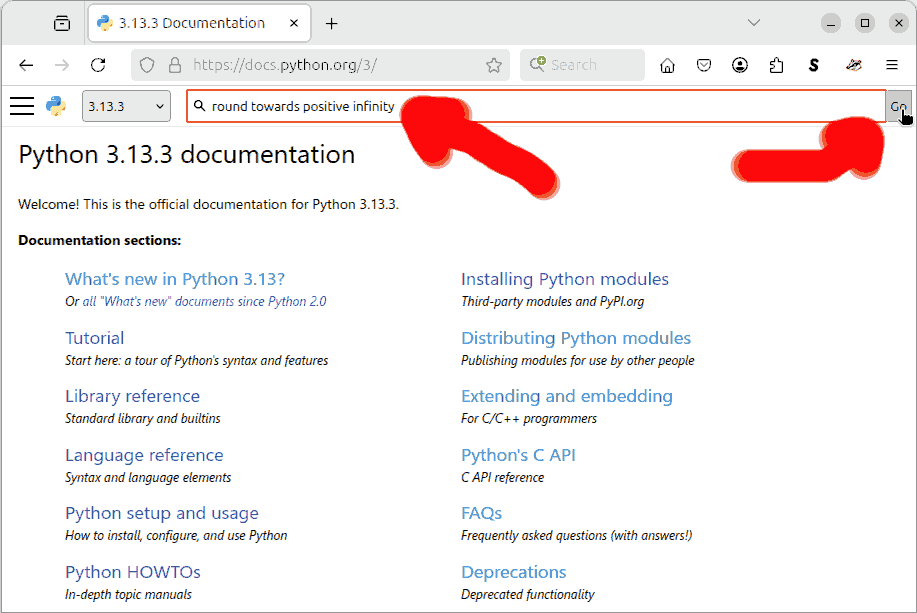
\includegraphics[width=0.47\linewidth]{\currentDir/rounding01searchInDocumentation}}}%
%
\floatSep%
%
\subfloat[][%
The results are not too useful. %
The first result is unrelated to floating point numbers. %
The second one is a complete list of all functions in the module~\pythonilIdx{math}. %
However, without knowing that the right function is called~\pythonilIdx{ceil}, finding it in this list could be hard.%
\label{fig:rounding02foundNothingUseful}%
]{\tightbox{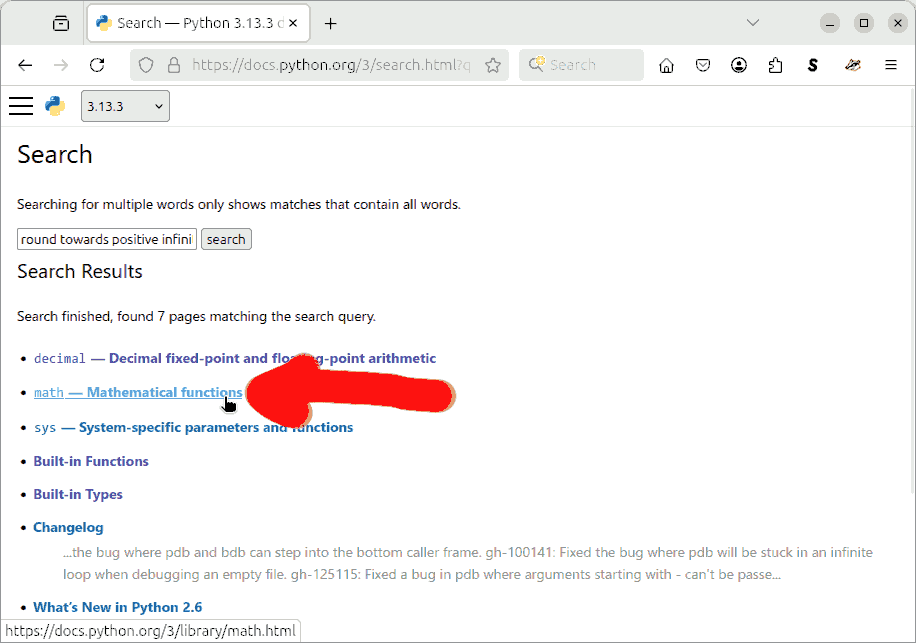
\includegraphics[width=0.47\linewidth]{\currentDir/rounding02foundNothingUseful}}}%
%
\floatRowSep%
%
\subfloat[][%
We enter \inQuotes{round towards positive infinity} into an internet search engine, here Microsoft Bing at~\url{https://bing.com}, but any search engine should do just as well. %
The result looks promising.%
\label{fig:rounding03searchEngine}%
]{\tightbox{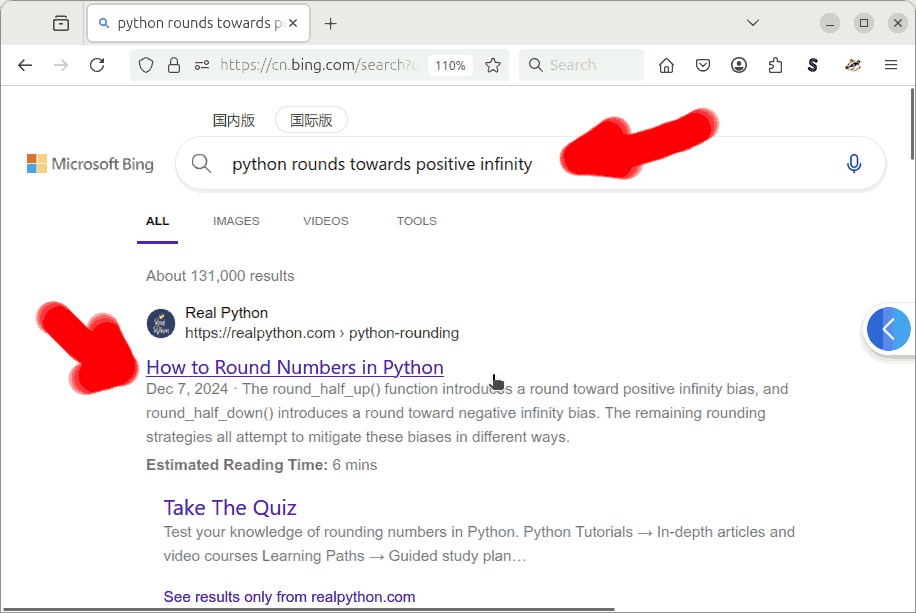
\includegraphics[width=0.47\linewidth]{\currentDir/rounding03searchEngine}}}%
%
\floatSep%
%
\subfloat[][%
Clicking on the first result, we visit the page~\citetitle{D2021RPT:A2024HTRNIP}~\cite{D2021RPT:A2024HTRNIP} at \citeurl{D2021RPT:A2024HTRNIP}.%
\label{fig:rounding04realPython}%
]{\tightbox{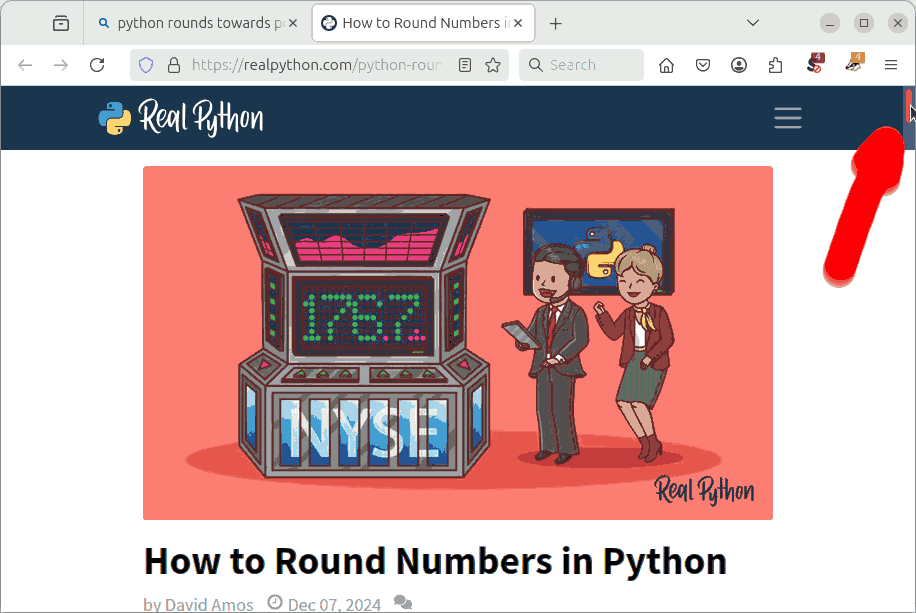
\includegraphics[width=0.47\linewidth]{\currentDir/rounding04realPython}}}%
%
\floatRowSep%
%
\subfloat[][%
After scrolling down a bit, we indeed find the information we want: %
For rounding up, the function~\pythonilIdx{ceil} is suitable. %
It is even presented as hyperlink.%
\label{fig:rounding05realPythonScrolledToCeil}%
]{\tightbox{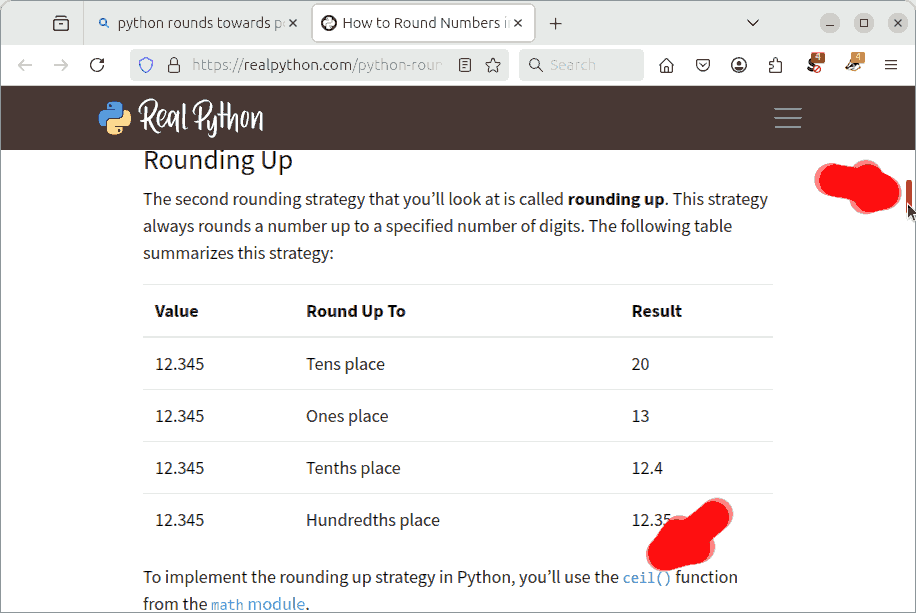
\includegraphics[width=0.47\linewidth]{\currentDir/rounding05realPythonScrolledToCeil}}}%
%
\floatSep%
%
\subfloat[][%
If we click on the hyperlink, it takes us to the \pythonilIdx{ceil}~entry in the \citetitle{PSF:P3D:TPSL:MMF} page~\cite{PSF:P3D:TPSL:MMF} at \citeurl{PSF:P3D:TPSL:MMF}.%
\label{fig:rounding06foundCeilInPythonDoc}%
]{\tightbox{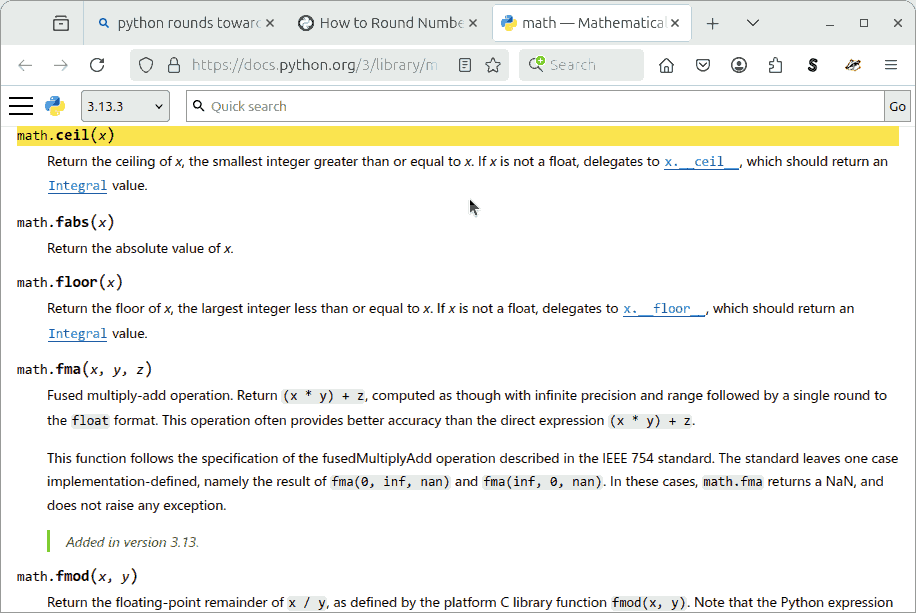
\includegraphics[width=0.47\linewidth]{\currentDir/rounding06foundCeilInPythonDoc}}}%
%
%
\caption{Searching for a \python\ function for \inQuotes{rounding up} if we do not know its name.}%
\label{fig:pythondoc:B}%
%
\end{figure}%
%
\begin{figure}%
\centering%
%
\subfloat[][%
The \citetitle{PSF:P3D:PSAU} page~\cite{PSF:P3D:PSAU} at~\citeurl{PSF:P3D:PSAU}.%
\label{fig:pythondocOther01setupAndUsage}%
]{\tightbox{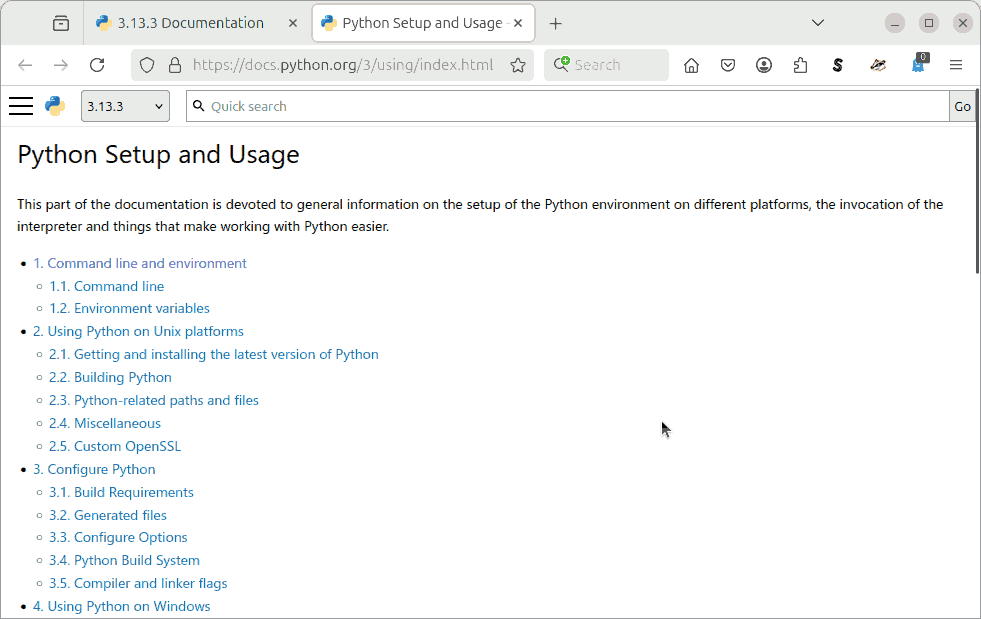
\includegraphics[width=0.47\linewidth]{\currentDir/pythondocOther01setupAndUsage}}}%
%
\floatSep%
%
\subfloat[][%
The \citetitle{PSF:P3D:TPT} page~\cite{PSF:P3D:TPT} page at~\citeurl{PSF:P3D:TPT}.%
\label{fig:pythondocOther02tutorial}%
]{\tightbox{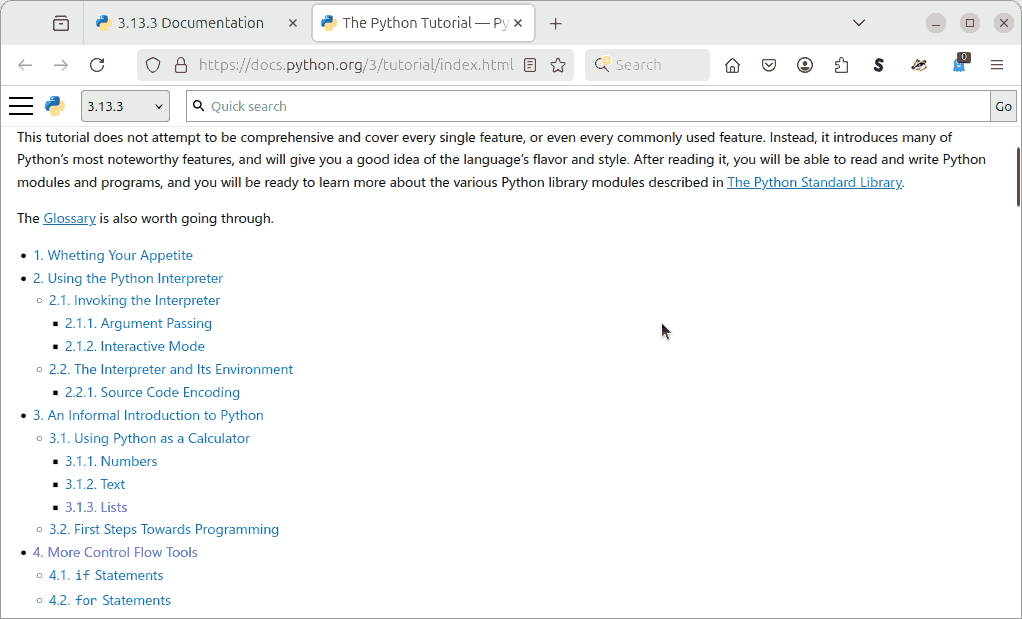
\includegraphics[width=0.47\linewidth]{\currentDir/pythondocOther02tutorial}}}%
%
\floatRowSep%
%
\subfloat[][%
The \citetitle{PSF:P3D:TPSL} page~\cite{PSF:P3D:TPSL} at~\citeurl{PSF:P3D:TPSL}.%
\label{fig:pythondocOther03standardLibrary}%
]{\tightbox{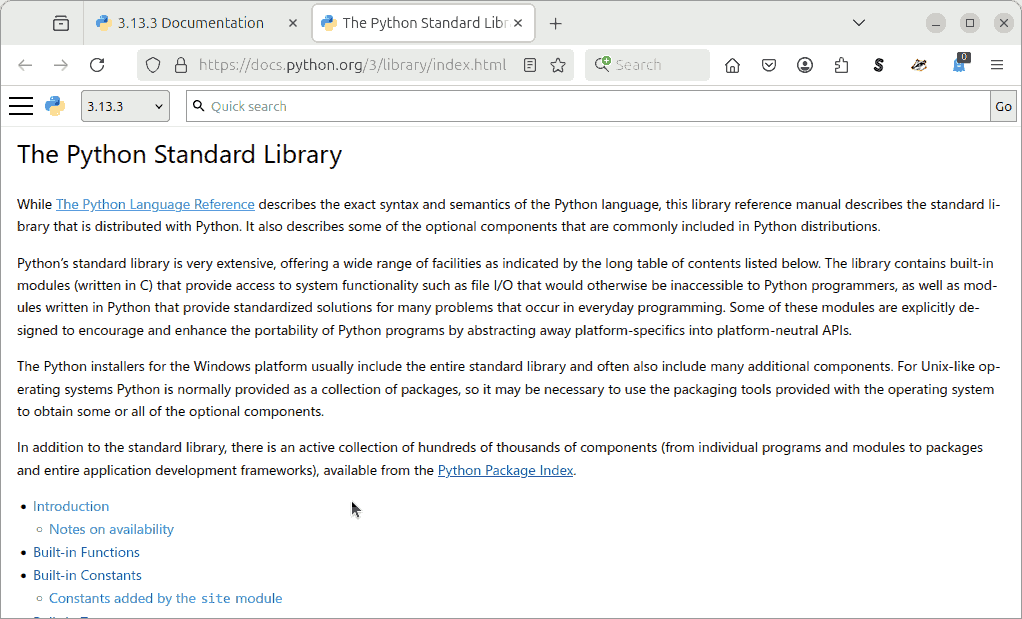
\includegraphics[width=0.47\linewidth]{\currentDir/pythondocOther03standardLibrary}}}%
%
\floatSep%
%
\subfloat[][%
The \citetitle{PEP0} page~\cite{PEP0} at~\citeurl{PEP0}.%
\label{fig:pythondocOther04pep0}%
]{\tightbox{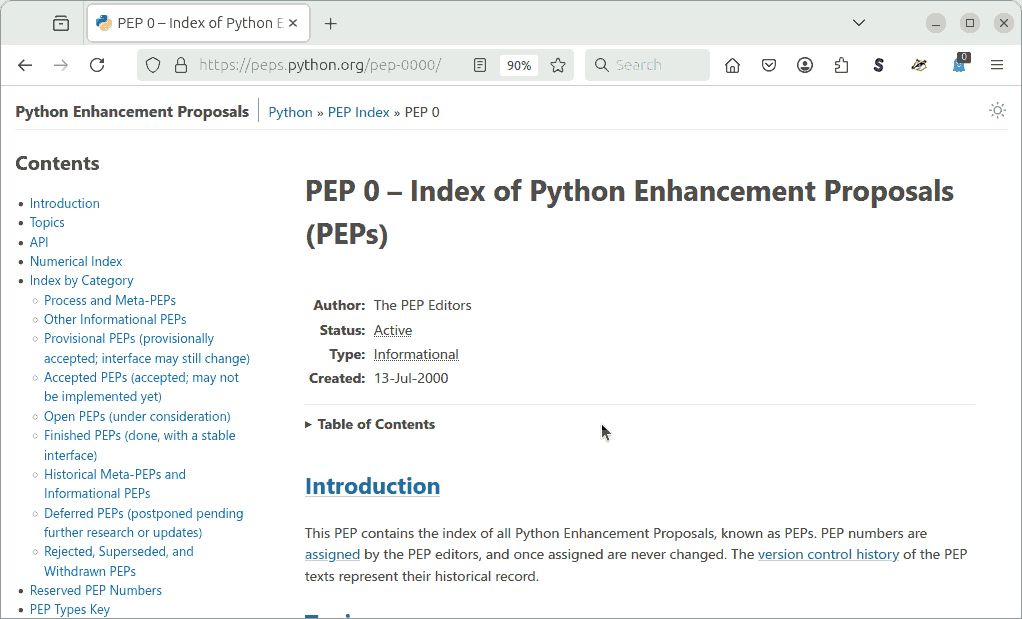
\includegraphics[width=0.47\linewidth]{\currentDir/pythondocOther04pep0}}}%
%
\caption{Several important authoritative online resources on \python.}%
\label{fig:pythondoc:C}%
\end{figure}%
%
In the previous section, we discussed lots of functions, \pythonilIdx{sin}, \pythonilIdx{cos}, \pythonilIdx{tan}, \pythonilIdx{atan}, \pythonilIdx{exp}, \pythonilIdx{log}, \pythonilIdx{round}, \pythonilIdx{floor}, \pythonilIdx{trunc}, and~\pythonilIdx{ceil}, to name just a few.
You could read about and explore what these functions do in this book.
However, there are two issues with this:

First, this book can only provide brief introductions into these functions from a didactic perspective.
It does not make any sense to here discuss their exact specifications and relationships to other functions in the \python\ ecosystem.
So what do you do if you need exact, authoritative information about full specification of a function?
Second, you only learn about the functions that we \emph{do} list.
What do you do if you want to learn about a function that we do not discuss here?

The answer to the first question is rather simple:
There is a complete online help catalog available for \python:~the \citetitle{PSF:P3D}~\cite{PSF:P3D} at~\url{https://docs.python.org/3}.
This should be your primary destination if you want to learn anything about \python.
Also, it is available in Chinese.

As example, let us imagine that you want to learn more about the function~\pythonilIdx{ceil}.
In \cref{fig:pythondoc01website}, we open a browser and visit the \citetitle{PSF:P3D}~\cite{PSF:P3D} at~\url{https://docs.python.org/3}.
On this page, you will either directly see a drop-down box where you can choose your favorite language or you can find it by clicking the \menu{\threeBarButton} at on the top-left corner of the website.
In the menu that opens in \cref{fig:pythondoc02language}, you can change the language and, e.g., select simplified Chinese~(简体中文) if that is your preferred language.
I will not do so and instead continue here in English.

Regardless of which language you chose, we still want to find information about the \pythonilIdx{ceil}~function.
Therefore, we locate the search bar \emph{in the website}~(not the one where you type in the \pglspl{URL} in the web browser).
Into this search bar, we type \pythonilIdx{ceil} and click on~\menu{Go} in \cref{fig:pythondoc03searchCeil}.

Depending on your internet connection and your location on the globe, it may take a bit of time until results are displaced.
Especially when visiting the page for the first time during a browsing session.
We wait patiently in \cref{fig:pythondoc04wait}.
And indeed, a list of documentation articles about the \pythonilIdx{ceil} function appears after a brief wait in \cref{fig:pythondoc05results}.
We decide that the link to \pythonil{math.ceil} looks most promising and click on it.

It takes us to the \pythonilIdx{ceil}~entry of the \citetitle{PSF:P3D:TPSL:MMF} page~\cite{PSF:P3D:TPSL:MMF} at \citeurl{PSF:P3D:TPSL:MMF}.
There, we find a brief explanation about the \pythonilIdx{ceil} function, as shown in \cref{fig:pythondoc06mathceil}.
The explanation also provides further reading, e.g., a link to the \dunder{ceil} method.
This is not important here, we will discuss it much later in~\cref{fig:pythonDunder:2}, but if we were interested, we could continue exploring and find more information about~\pythonilIdx{ceil}.
Also, we see that the information about the \pythonilIdx{ceil}~function is part of a longer list of mathematical functions.
Being curious, we would scroll a bit through this list.
Maybe we could learn about one or two other functions that we did not know about yet.%
%
\usefulTool{pythonDoc}{%
The first place to look for information about \python\ is the official \citetitle{PSF:P3D} at \citeurl{PSF:P3D}. %
This is the \emph{authoritative} source about \python: %
Everything what is written there is \emph{true} and \emph{exact} regarding~\python. %
All other sources may contain errors, be imprecise, ambiguous, or outdated. %
Therefore, always first consult the official \python\ documentation when being in doubt or looking for information.%
}%
%
Of course, in many cases, we do not know the name of the function we are looking for.
Assume that you did not know that the function~\pythonilIdx{ceil} exists.
You were looking for a way to round floating point numbers \inQuotes{upwards.}

You want to do something that you know should somehow be possible.
You think that \python\ should probably offer some out-of-the-box function for doing that.
If not, there should at least be some \inQuotes{standard \python way} to do that.
Anyway, the point is:
You do not have a function name to look for.

Let's again start at the search mask of the \citetitle{PSF:P3D} at~\citeurl{PSF:P3D}.
In \cref{fig:rounding01searchInDocumentation}, we try to describe what we want to do as clearly as possible.
\inQuotes{Rounding up} is maybe not very precise.
Let's enter \inQuotes{round towards positive infinity} into the search mask.

Sadly, the results shown in \cref{fig:rounding02foundNothingUseful} are not too useful.
This can happen.
The first result is unrelated to floating point numbers.
It offers us some discussion about objects implementing fractional arithmetics in a different way.
While we could find some hints in this text, it is not useful.

The second search result takes us to the a complete list of all functions in the module~\pythonilIdx{math}~\cite{PSF:P3D:TPSL:MMF}, but \emph{not} to the \pythonilIdx{ceil} function.
This means that we would need to go through the whole list of functions, read all of their descriptions, until we arrive at one that matches our goals.
This is a feasible method.
The list is not too long.
We could indeed spot the right answer here.
And we would probably learn more about \python\ on the way.
So directly working our way through the documentation here is a good idea.

But let's say that we did not find anything useful and gave up using the \python\ documentation directly.
The second thing that we could try is to enter the description of what we want to do into a common search engine.
In \cref{fig:rounding03searchEngine}, we use Microsoft Bing at~\url{https://bing.com}, but any other search engine would probably be as same as good.
We enter \inQuotes{round towards positive infinity} into the search mask and hit~\menu{Search}.

The first result looks promising right way.
\inQuotes{\cite{D2021RPT:A2024HTRNIP}} {\dots} while it does not say \inQuotes{round towards infinity,} if it summarizes all information about rounding numbers, that topic is bound to come up somewhere.
So we click the link.

It takes us visit to the page~\citetitle{D2021RPT:A2024HTRNIP}~\cite{D2021RPT:A2024HTRNIP} at \citeurl{D2021RPT:A2024HTRNIP} in \cref{fig:rounding04realPython}.
A summary page on all about rounding of numbers.
Nice.

We begin to read the text.
Reading is an important skill, as reading texts and tutorials can significantly expand our knowledge.
After reading for a while, we indeed find the information we want:
For rounding up, the function~\pythonilIdx{ceil} is suitable.
It is even presented as a hyperlink in \cref{fig:rounding05realPythonScrolledToCeil}.
If we click on the hyperlink in \cref{fig:rounding06foundCeilInPythonDoc}, it takes us to the \pythonilIdx{ceil}~entry in the \citetitle{PSF:P3D:TPSL:MMF} page~\cite{PSF:P3D:TPSL:MMF} at \citeurl{PSF:P3D:TPSL:MMF}.
So we went round trip:
Even if we do not know how to do a given thing or what its name is, we can still find our way to the \python\ documentation.%
%
\usefulTool{searchEngines}{%
Search engines are useful tools to find information about certain functionality. %
Writing a precise description of the problem or functionality into the search bar of a search engine can lead to pages that describe answers or take us to the official \python\ documentation. %
However, search engines can also lead us to pages containing wrong, incomplete, ambiguous, outdated, or otherwise useless information. %
It is important to compare whatever information we found with the official \python\ documentation~\cite{PSF:P3D}.%
}%
%
Let us also note:
Besides being a source of authoritative information about \python, the official website also offers a variety of other useful information.
You may have already used the \citetitle{PSF:P3D:PSAU} page~\cite{PSF:P3D:PSAU} at~\citeurl{PSF:P3D:PSAU}, screenshotted in \cref{fig:pythondocOther01setupAndUsage}, when installing \python\ on your system.

The \citetitle{PSF:P3D:TPT} page~\cite{PSF:P3D:TPT} page at~\citeurl{PSF:P3D:TPT} and shown in \cref{fig:pythondocOther02tutorial} offers several useful tutorials.
Actually, it describes many of the techniques that we discuss in this book in much depth and very nicely, probably even better than this book.
I very strongly urge you to also read this website.

The \citetitle{PSF:P3D:TPSL} page~\cite{PSF:P3D:TPSL} at~\citeurl{PSF:P3D:TPSL} depicted in \cref{fig:pythondocOther03standardLibrary} contains the specification of all the standard functions that ship with \python.
It is therefore a very useful tool when checking what a function \emph{actually} does, to complement our learned knowledge.

Finally, the \citetitle{PEP0} page~\cite{PEP0} at~\citeurl{PEP0} shown in \cref{fig:pythondocOther04pep0} contains all changes and additions to the \python\ language since roughly the year~2000.
We can find many of the language utilities that we are using in this book defined in a so-called~\emph{Python Enhancement Proposal~(PEP)}.%
%
\FloatBarrier%
\global\let\glslink\oldinterludepythonglslink%
\endhsection%
%
